\section{The problem}
\label{sec:problem}

Experts leave out the reasoning steps that have become automatic for them.
The whole project builds on this premise, so this section states what the
evidence shows, at what scale and in which domains.

\subsection{Why experts leave knowledge out}

Practice compiles a sequence of decisions into a single, fast, automatic
procedure, and the compiled procedure no longer needs the declarative
knowledge it was built from \parencite{anderson1982acquisition}. \evlit\ Once
a skill reaches this state, its steps are, in a phrase repeated across the
cognitive-task-analysis literature, ``not available for introspection''
\parencite[p.~584]{clark2008cognitive}. An expert asked to explain a familiar
task therefore omits the steps that no longer need conscious attention, not
out of reticence but because those steps no longer come to mind unprompted.
Feldon draws out what this implies for teaching
\parencite{feldon2007implications,feldon2007cognitive}. How much any one
report leaves out is an empirical question.

\subsection{What omission looks like when it is measured}

\begin{evlitbox}
  Three surgeons, videotaped teaching a cricothyrotomy, were compared
  against a 46-step task list built by cognitive task analysis from three
  other surgeons. On average, they omitted 71\% of clinical-knowledge steps
  (10 of 14), 51\% of action steps (14 of 27), and 73\% of decision steps
  (3.6 of 5). They described \emph{how} to perform the step for only 13\%
  of action steps (3.6 of 27) \parencite{sullivan2014use}. Directed
  cognitive-task-analysis prompting raised the average share of steps each
  surgeon described in the CTA interview from 44\% (20 of 46) to 66\%
  (31 of 46).
\end{evlitbox}

\evlit\ Two other studies give numbers. In programming, six expert
programmers explained their troubleshooting under several elicitation
methods, and the share of procedural knowledge acquired roughly doubled from
one expert to six \parencite{chao1994percentage}. A review reports the
detail: no single expert reported more than 41\% of diagnostic actions,
53\% of debugging actions, or 29\% of interpretations under any elicitation
method, and pooling all six raised coverage to 87\%, 88\%, and 62\%
\parencite[p.~585]{clark2008cognitive}. In nursing, Critical Decision
Method interviews with neonatal intensive-care nurses elicited significantly
more information than non-CDM interviews, and produced a sepsis-assessment
guide with information ``not available in the current literature''
\parencite{crandall1993critical}; the same review reports 17 nurses
\parencite[p.~584]{clark2008cognitive}. The often-repeated ``25 of 70 cues''
also comes from that review \parencite[p.~585]{clark2008cognitive}.

These studies do not license a single omission rate. Each has 3 to 17
experts in one domain, and their gold standards are themselves built by
cognitive task analysis, which makes the comparison partly circular.
\evint\ A figure often quoted outside this literature, that experts are
unaware of about 70\% of their own decisions, is not a new measurement:
\textcite[p.~591]{clark2008cognitive} state it citing two earlier review
chapters. We treat the direction of the effect as established: experts omit
a large, variable share of decisions, cues and interpretations. Any specific
rate beyond the cited studies is unsupported.

\begin{figure}[tbp]
  \centering
  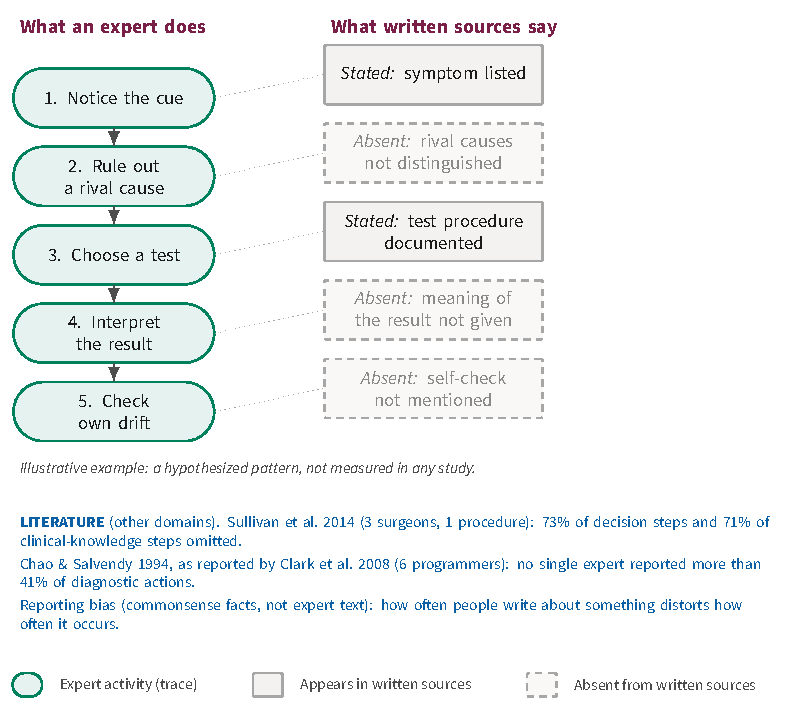
\includegraphics{figures/pdf/fig01_problem.pdf}
  \caption[What reaches text, and what does not]{What part of expert
    knowledge reaches text, and what does not. Automaticity, measured
    omission in three small studies, and reporting bias in written text
    explain why the overlap between ``what an expert knows'' and ``what an
    expert or a writer states'' is partial, and concentrated away from
    decisions, cues and interpretations.}
  \label{fig:problem}
\end{figure}

\subsection{Reporting bias: writers omit the obvious too}

\evlit\ Writers omit the obvious too: how often people write about actions,
outcomes and properties systematically distorts how often they occur
\parencite{gordon2013reporting}. Text-only language models inherit the
distortion, for example in the colors they predict for 521 objects
\parencite{paik2021world}. \evint\ Omission in speech and
reporting bias in text point at the same target: cues, decisions,
interpretations, checks and the boundaries of hedged rules, not the parts of
a domain already stated as principles or procedures.

\subsection{One education example: principle selection}

\evlit\ Experts sort physics problems by the principle that solves them
(conservation of energy, Newton's second law); novices sort the same
problems by surface features such as ``inclined-plane problems''
\parencite{chi1981categorization}. Naming the governing principle is an
expert operation that an expert does not think to state, because for the
expert it happens as recognition, not as a step. Experts do not just omit
their own principle-selection step; in the blind-spot studies reviewed in
\cref{sec:foundations-learners}, their predictions of what novices find hard
were well above chance but far from complete, and more expertise did not
improve them. Hence the education path
(\cref{sec:education}) never treats an expert's or an AI's guess about
learner difficulty as evidence.

\subsection{One organizational example: the copier technician's story}

\begin{evlitbox}
  Orr's ethnography of photocopier repair technicians found that diagnosis
  runs through narrative: technicians build and circulate a coherent story
  of how a machine is actually failing. That story, not the service
  manual, keeps the group's diagnostic knowledge current
  \parencite{orr1996talking}. Brown and Duguid read it as knowledge held by a
  community of practice \parencite{brown1991organizational}.
\end{evlitbox}

The manual describes the machine as designed; the technicians' story
describes it as it fails. \evobs\ Run on public troubleshooting text for
programmable logic controllers, the N3 gap map produced a record of the same
shape from the span ``a common mistake\dots\ is panicking and abandoning
systematic approaches.'' The sources name the failure mode, and the absence
check found at most a partial statement of how a troubleshooter notices the
drift into it (state: \code{partial}).\footnote{%
  \repo{research/n3/plc/gapmap.json}, the GUARD-lens record at rank 9.}
This shows only that a lens can flag text of this \emph{shape}; nothing
confirms that the item is real tacit knowledge, and the absence check is not
yet informative (\cref{sec:n3}).

\subsection{Why this matters}

The omission that makes a domain hard to teach also makes it expensive to
transfer inside an organization. \evlit\ Transfer of best practice
inside firms is blocked mainly by the recipient's capacity to absorb it and
by causal ambiguity, not by unwillingness to share
\parencite{szulanski1996exploring}. Software engineering shows what this costs when a
person who holds the knowledge leaves: many popular open-source projects
depend on one or two developers \parencite{avelino2016novel}. Turnover then
exposes projects to losses far above the expected loss
\parencite{rigby2016quantifying,nassif2017revisiting}
(\cref{sec:organizations}). \evint\ Training, onboarding and succession all
fail when such knowledge is not made explicit before its holder leaves.

\subsection{What AI changes, and what it does not}

An AI system can read far more sources than a person and keep a checkable
link from each claim to its supporting sentence (\cref{sec:approach}).
\evint\ What it cannot do is see past the wall the omission
and reporting-bias evidence describes: a language model trained on text
inherits the silences of that text \parencite{paik2021world}. An AI system
can make the boundary between what is written and what is not sharper and
more auditable, and it can flag the shape of a likely silence using the
constructs in \cref{sec:foundations}. It cannot tell on its own whether a
flagged silence hides real expert knowledge, a fact nobody happened to write
down, or nothing. That needs a human answer, which is why every output of
the pipeline carries an evidence label (\cref{sec:evidence-model}) and why
\code{inferred} never reads as \code{observed_human_evidence}.
